\chapter{State of the union}\label{state-of-the-union}

The previous chapter quickly introduces the basic notions of RP. This
chapter will give an overview of the state of the art for RP frameworks.

This thesis author arbitrarily choose four relevant libraries:

\begin{itemize}
\itemsep1pt\parskip0pt\parsep0pt
\item
  Scala.React
\item
  RxJava
\item
  ReactiveCocoa
\item
  Akka Streams
\end{itemize}

\section{Scala.React}\label{scala.react}

\textbf{Scala.React} is a framework that has been introduced with the
paper ``Deprecating the Observer Pattern'' from Maier, Odersky and
Rompf. The key concepts around Scala.React originate in Elliot's FRP,
and Scala.React aims to provide a \textbf{combinator-based approach for
reactive programming}.

The paper depicts how the observer pattern should be considered an
anti-pattern, since it violates a lot of software engineering principles
such as encapsulation, composability, separation of concerns,
scalability, uniformity, abstraction, semantic distance..

The authors aims to provide and depict an efficient use of
object-oriented, functional, and data-flow programming principles to
overcome the limitations of the existing approaches.

After many years from its presentation, the framework seems to be an
academic library that can be neglectable in favor of the RxScala/RxJava
library. For the author of this thesis, the paper is really meaningful
in the context of this thesis, since it introduces a set of abstractions
that are close to the original model of FRP from Elliot.

\subsection{Reactive}\label{reactive}

Following the idea to provide APIs that starts with basic event handling
and ends in an embedded higher-order dataflow language, the framework
introduces a generic trait \texttt{Reactive}, that factors out the
possible concrete abstractions in the following way:

\begin{verbatim}
trait Reactive[+Msg, +Now] {
    def current(dep: Dependant): Now
    def message(dep: Dependant): Option[Msg]
    def now: Now = current(Dependent.Nil)
    def msg: Msg = message(Dependent.Nil)
}
\end{verbatim}

The trait \texttt{Reactive} is defined based on two type parameters: one
for \textbf{the message type an instance emits} and one for \textbf{the
values it holds}.

Starting from the previous base abstraction, two further types can be
defined:

\begin{verbatim}
trait Signal[+A] extends Reactive[A,A]
trait Events[+A] extends Reactive[A,Unit]
\end{verbatim}

The difference between the two types can be seen directly in the types:

\begin{itemize}
\itemsep1pt\parskip0pt\parsep0pt
\item
  In \texttt{Signal}, \texttt{Msg} and \texttt{Now} types are identical.
\item
  In \texttt{Events}, \texttt{Msg} and \texttt{Now} types differ. In
  particular, the type for the type parameter \texttt{Now} is
  \texttt{Unit}. This means that for an instance of \texttt{Events} the
  notion of ``current value'' has no sense at all.
\end{itemize}

The two subclasses need to implement two methods, which obtain reactive's current message or value and create dependencies in a single
turn.

The next two sections will better examine the two abstraction introduced
here.

NB: the examples and code provided in this chapter have been taken
directly from the paper itself.

\subsubsection{Events}\label{events}

The first type to take in consideration is the \texttt{Event} type.

To simplify the event handling logic in an application, the framework
provides a general and uniform event interface, with
\texttt{EventSource}. An \texttt{EventSource} is an entity that can
\emph{raise} or \emph{emit} events at any time. For example:

\begin{verbatim}
val es = new EventSource[Int]
es raise 1
es raise 2
\end{verbatim}

To attach a side-effect in response to an event, an observer has to
\emph{observe} the event source, providing a closure. Continuing with
the previous example, the following code prints all events from the
event source to the console.

\begin{verbatim}
val ob = observe(es) { x =>
    println("Receiving " + x)
}
...
ob.dispose()
\end{verbatim}

\texttt{observe(\ )} returns an handle of the observer,that can be used
to uninstall and dispose the observer prematurely, via its
\texttt{dispose()} method. This is a common pattern in all of the other
frameworks/libraries presented in this thesis.

The basic types for events handling are pretty neat and simple to reason
about, since they are first-class values. The usage of these types
starts to be helpful only if combined with a set of operators, that
enables developers to build better and declarative abstraction.

For example, the \texttt{Events} trait defines some common operators as
follows:

\begin{verbatim}
def merge[B>:A](that: Events[B]): Events[B]
def map[B](f: A => B): Events[B]
def collect[B](p: PartialFunction[A, B]): Events[B]
\end{verbatim}

When building abstractions, the developer doesn't need to take care of
the events propagation, since the framework itself provides this.

\subsubsection{Signal}\label{signal}

The \textbf{Signal} type represents the other half of the story.

In programming a large set of problems is about \textbf{synchronizing
data that changes over time}, and signals are introduced to overcome
these needs.

In simple words, a \texttt{Signal} is the \textbf{continuous}
counterpart of trait \texttt{Events} and represents \textbf{time-varying
values}, maintaining:

\begin{itemize}
\itemsep1pt\parskip0pt\parsep0pt
\item
  its \textbf{current value}
\item
  the current \textbf{expression} that defines the signal value
\item
  a set of \textbf{observers}: the other signals that depend on its
  value
\end{itemize}

A concrete type for \texttt{Signal} is the \texttt{Var}, that abstract
the notion of \textbf{variable signal} and is defined as follows:

\begin{verbatim}
class Var[A](init: A) extends Signal[A] {
    def update(newValue: A): Unit = ...
}
\end{verbatim}

A \texttt{Var}'s current value can change when somebody calls an
\texttt{update(\ )} operation on a it or the value of a dependant signal
changes.

\textbf{Constant signals} are represented by \texttt{Val}:

\begin{verbatim}
class Val[A](value: A) extends Signal[A]
\end{verbatim}

To compose signals, the framework doesn't provide combinator methods at
all, but introduce the notion of \textbf{signal expressions}, indeed. To
better explain the concept, let's look at a simple example.

\begin{verbatim}
val a = new Var(1)
val b = new Var(2)
val sum = Signal{ a()+b() }

observe(sum) { x => println(x) }

a()= 7
b()= 35
\end{verbatim}

Signals are primarily used to create variable dependencies as seen
above. In other words, the framework itself already performs all the “plumbing work” of connecting the dependencies and propagating the changes.

The framework and the Scala language provide a convenient and simple
syntax to get and update the current value of a Signal, and also to
create variable dependencies between signals. For example:

\begin{itemize}
\itemsep1pt\parskip0pt\parsep0pt
\item
  the code \texttt{Signal\{\ a()+b()\ \}} creates a dependencies that
  binds the changes from \texttt{a} and \texttt{b} to be propagated and
  evaluated in the \texttt{sum} signal
\item
  the code \texttt{a()=\ 7} is evaluated as \texttt{a.update(7)}
\item
  the framework also provide an implicit converter that enables to
  create easily \texttt{Val} signals
\end{itemize}


\subsection{Evaluation model}\label{evaluation-model}

Scala.React's propagation model is \textbf{push-driven}, and uses a
\textbf{topologically ordered dependency graph}. This implementation
detail ensures that an expression is always evaluated after all its
dependants have been evaluated, so glitches can't happen.

Scala.React proceeds in \textbf{propagation cycles}. The system is
\emph{either in a propagation cycle or}, if there are no pending changes
to any reactive, \emph{idle}. The model of \textbf{time} the system use
is a \textbf{discrete} one.

Every propagation cycle has two phases: first, all reactives are
synchronized so that observers, which are run in the second phase,
cannot observe inconsistent data. During a propagation cycle, the
reactive world is paused, i.e., no new changes are applied and no source
reactive emits new events or changes values.

A propagation cycle proceeds as follows:

\begin{enumerate}
\def\labelenumi{\arabic{enumi}.}
\itemsep1pt\parskip0pt\parsep0pt
\item
  Enter all modified/emitting reactives into a priority queue with the
  priorities being the reactives' levels.
\item
  While the queue is not empty, take the reactive on the lowest level
  and validate its value and message. The reactive decides whether it
  propagates a message to its dependents. If it does so, its dependents
  are added to the priority queue as well.
\end{enumerate}

\section{RxJava}\label{rxjava}

The table represents a possible classification of the
\textbf{effects} in programming.

\begin{table}[]
\centering
\caption{The essential effects in programming}
\label{my-label}
\begin{tabular}{|l|l|l|}
\hline
             & {\bf One}     & {\bf Many}        \\ \hline
Synchronous  & T/Try{[}T{]}  & Iterable{[}T{]}   \\ \hline
Asynchronous & Future{[}T{]} & \textbf{Observable{[}T{]}} \\ \hline
\end{tabular}
\end{table}

All the theory and the development of the reactive extensions libraries
started with an intuition of Erik Meijer, that theorized that
\textbf{iterable/iterator} are \textbf{dual} to
\textbf{observable/observer}. And this hypothesis is what let us to
relate all the principal effects in programming, where in one axis
there's is the nature of the computation (sync or async) and in the
other one there's the cardinality of the result (one or many).

The appendix on \textbf{futures and promises} covers the case of a
computation that returns a \textbf{single value}. This chapter will
focus on the abstraction of \textbf{Observables}, analyzing RxJava as a
case of study.

As the title of the repository states, \emph{RxJava is a library for
composing asynchronous and event-based programs using observable
sequences for the JVM}.

The library was heavily inspired by Rx.NET by Microsoft and is
developed by Netflix and other contributors. The code is open source
and recently, after 2 years of development, has reached the 1.0 version.

RxJava is also conform to the Reactive Streams initiative (see the
appendix), and this means that the hard problem of propagating and
reacting to back-pressure has been incorporated in the design of RxJava
already, and also that it interoperate seamlessly with all other
Reactive Streams implementations.

\subsection{Observable}\label{observable}

The fundamental entity of RxJava is the \textbf{Observable} type. An
observable is a \emph{sequence of ongoing event ordered in time}.

An \texttt{Observable} can emit 3 types of item:

\begin{itemize}
\itemsep1pt\parskip0pt\parsep0pt
\item
  values
\item
  error
\item
  completion event
\end{itemize}

RxJava provides a really nice documentation, with also some graphical
diagrams, called marble diagrams.

\begin{figure}[htbp]
\centering
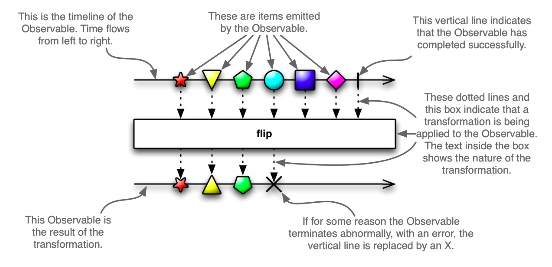
\includegraphics[scale=0.75]{imgs/marble.png}
\caption{A marble diagram}
\end{figure}

A marble diagram depicts how a an \texttt{Observable} and an
\texttt{Operator} behave:

\begin{itemize}
\itemsep1pt\parskip0pt\parsep0pt
\item
  observables are timelines with sequence of symbols
\item
  operators are rectangles, that accepts in input the upper observable
  and return in output the lower one
\end{itemize}

In RxJava, an \texttt{Observable} is defined over a generic type
\texttt{T}, the type of its values, as follows:

\begin{verbatim}
class Observable<T> { ... }
\end{verbatim}

An \texttt{Observable} can emit - in order - \textbf{zero, one or more
values, an error or a completion event}.

An \texttt{Observable} is an \textbf{immutable} entity, so the only way
to change the sequence of values it emits is through the application of
an \textbf{operator} and the subsequent creation of a new
\texttt{Observable}.

An entity can subscribe its interest in the values coming from an
\texttt{Observalbe} through its \texttt{subscribe(\ )} method, that
accepts one, two or three \texttt{Action} parameters (that correspond to
the \texttt{onNext(\ )}, \texttt{onError(\ )} and
\texttt{onComplete(\ )} callbacks).

The classic ``Hello, World'' example in RxJava and Java 8 is the
following:

\begin{verbatim}
Observable.just("Hello, world!").subscribe(s -> System.out.println(s));
\end{verbatim}

The \texttt{Observable} type provides some convenience methods that
return an observable with the given specification. An incomplete list
of these is the following:

\begin{itemize}
\itemsep1pt\parskip0pt\parsep0pt
\item
  \texttt{just(\ )}: convert an object or several objects into an
  Observable that emits that object or those objects
\item
  \texttt{from(\ )}: convert an Iterable, a Future, or an Array into an
  Observable
\item
  \texttt{empty(\ )}: create an Observable that emits nothing and then
  completes
\item
  \texttt{error(\ )}: create an Observable that emits nothing and then
  signals an error
\item
  \texttt{never(\ )}: create an Observable that emits nothing at all
\item
  \texttt{create(\ )}: create an Observable from scratch by means of a
  function
\item
  \texttt{defer(\ )}: do not create the Observable until a Subscriber
  subscribes; create a fresh Observable on each subscription
\item
  \ldots{}
\end{itemize}

Usually, observables created with these methods are used in conjunction
with other observables and operators, to create more complex logics.

\subsubsection{Operator}\label{operator}

In RxJava, operators are what enable the developer to \textbf{model} the
actual computation. An operator allows performing \textbf{almost every
type of manipulation} on the source observer in a declarative way.

Expressing a computation in terms of a stream of values is translated in
building a \textbf{chain of proper operators}. Usually, looking at the
signatures and at the types of the operators is really helpful when
choosing which operator is the right one for the goal to achieve.

An operator, to be applicable to an Observable, has to implement the
\texttt{Operator} interface and has to be lifted. The \texttt{lift}
function lifts a function (inside an \texttt{Operator}) to the current
Observable and returns a new Observable that when subscribed to will
pass the values of the current Observable through the \texttt{Operator}
function.

Operators are methods of the \texttt{Observable} class, so creating a
chain of operators starting from a source observable is a pretty
straightforward process.

RxJava provides a huge set of operators, and a lot of them is defined
in terms of other ones. What follows is only a small introductive
subset.

\subsubsubsection{Map}\label{map}

\texttt{Map} is an operator that returns an Observable that
\textbf{applies a specified function to each item} emitted by the source
Observable and emits the results of these function applications. Its
marble diagram is the following.

\begin{figure}[htbp]
\centering
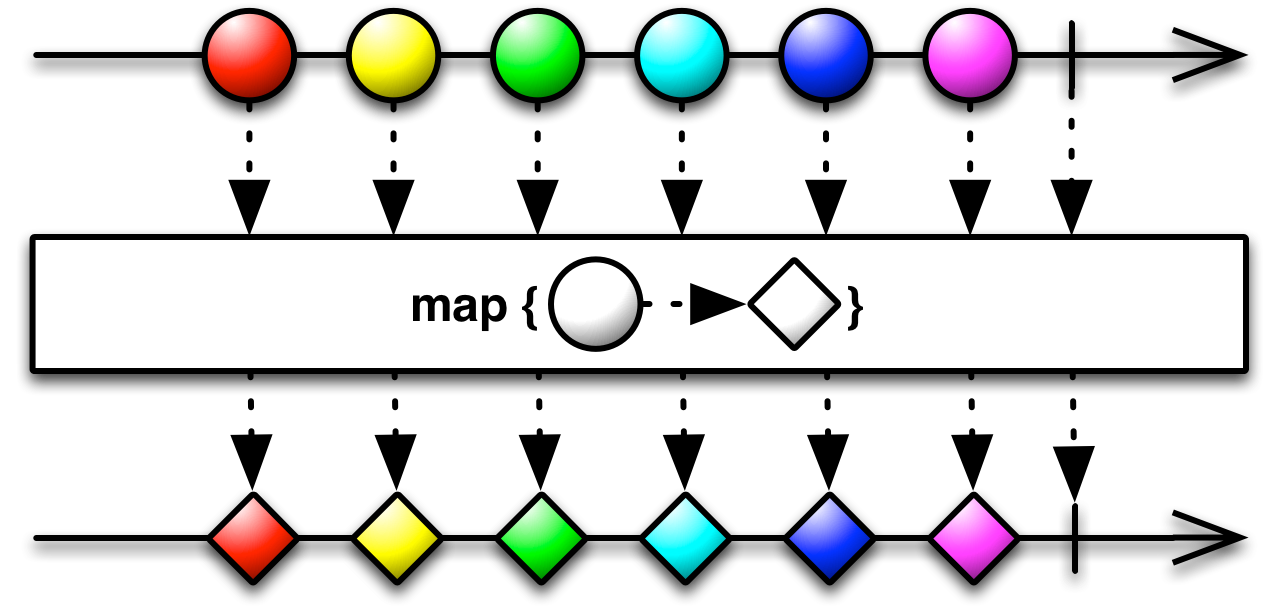
\includegraphics[scale=0.5]{imgs/map.png}
\caption{Map operator}
\end{figure}

To better clarify the concept of lifting introduced previously, let's
also look at the definition and implementation for \texttt{Map}.

\begin{verbatim}
public final <R> Observable<R> map(Func1<? super T, ? extends R> func) {
  return lift(new OperatorMap<T, R>(func));
}

...

public final class OperatorMap<T, R> implements Operator<R, T> {

    private final Func1<? super T, ? extends R> transformer;
    public OperatorMap(Func1<? super T, ? extends R> transformer) {
        this.transformer = transformer;
    }

    public Subscriber<? super T> call(final Subscriber<? super R> o) {
        return new Subscriber<T>(o) {

            public void onCompleted() {
                o.onCompleted();
            }

            public void onError(Throwable e) {
                o.onError(e);
            }

            public void onNext(T t) {
                try {
                    o.onNext(transformer.call(t));
                } catch (Throwable e) {
                    onError(OnErrorThrowable.addValueAsLastCause(e, t));
                }
            }
        };
    }
}
\end{verbatim}

\subsubsubsection{FlatMap}\label{flatmap}

\texttt{FlatMap} returns an Observable that \textbf{emits items based on
applying a function that is supplied to each item emitted by the source
Observable, where that function returns an Observable}, and then merging
those resulting Observables and emitting the results of this merger.

\begin{figure}[htbp]
\centering
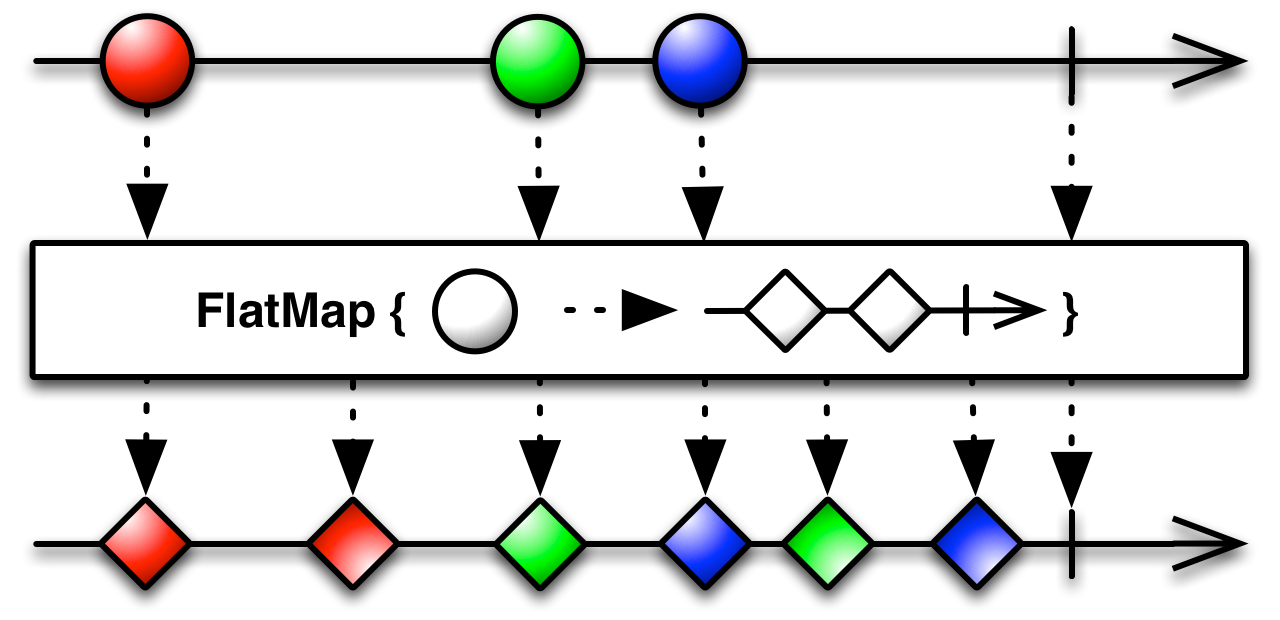
\includegraphics[scale=0.5]{imgs/flatMap.png}
\caption{FlatMap operator}
\end{figure}

\subsubsubsection{Filter}\label{filter}

\texttt{Filter} is quite obvious.

\begin{figure}[htbp]
\centering
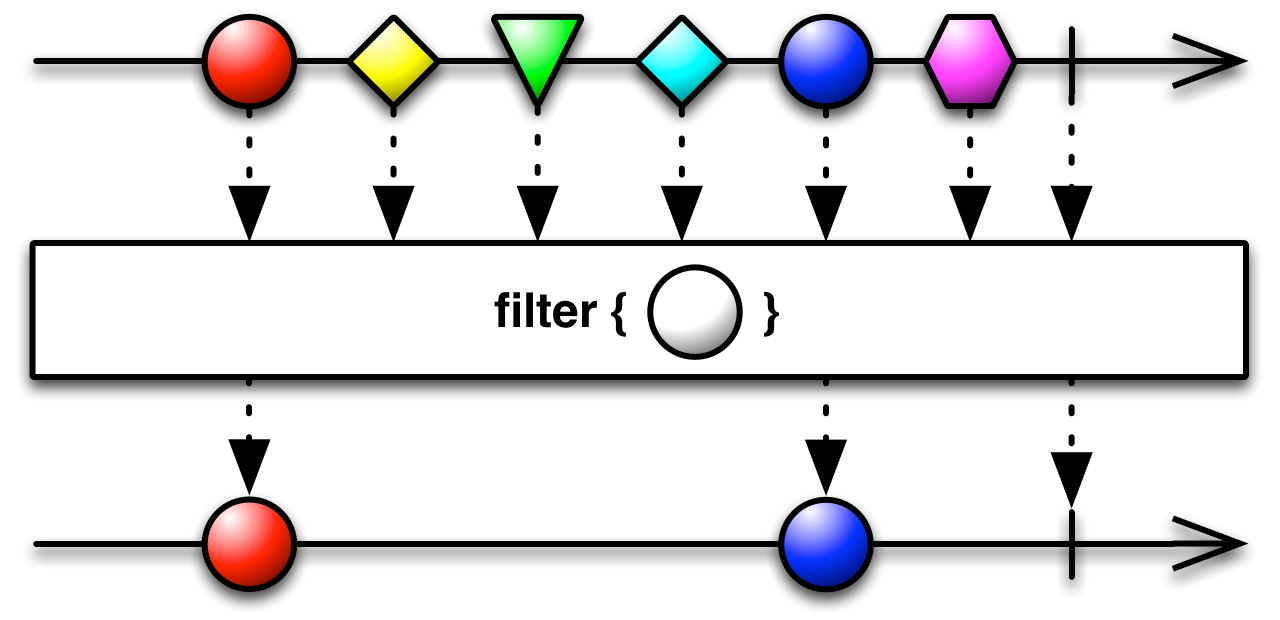
\includegraphics[scale=0.5]{imgs/filter.png}
\caption{Filter operator}
\end{figure}

\subsubsubsection{Scan}\label{scan}

\texttt{Scan} returns an Observable that \textbf{applies a specified
accumulator function} to the first item emitted by a source Observable,
then \textbf{feeds the result of that function along} with the second
item emitted by the source Observable into the same function, and so on
until all items have been emitted by the source Observable, and emits
the final result from the final call to your function as its sole item.

\begin{figure}[htbp]
\centering
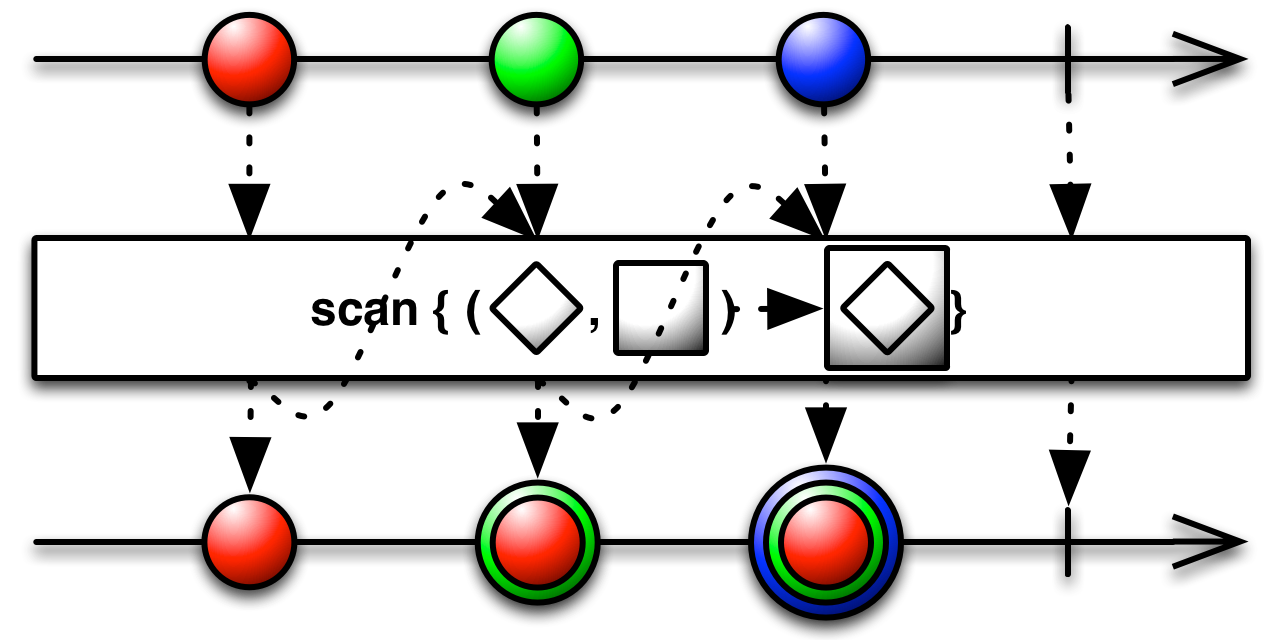
\includegraphics[scale=0.5]{imgs/scan.png}
\caption{Scan operator}
\end{figure}

\subsubsubsection{Take}\label{take}

\texttt{Take} returns an Observable that emits only the first n items
emitted by the source Observable.

\begin{figure}[htbp]
\centering
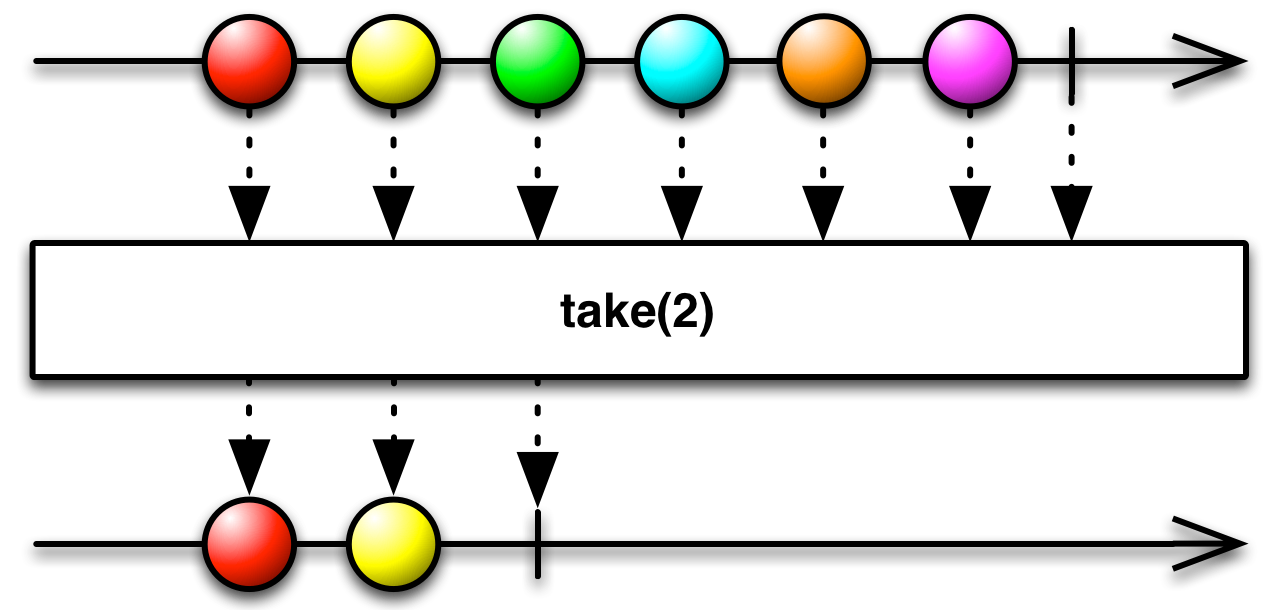
\includegraphics[scale=0.5]{imgs/take.png}
\caption{Take operator}
\end{figure}

\subsubsubsection{A complex example}\label{a-complex-example}

\begin{verbatim}
// Returns a List of website URLs based on a text search
Observable<List<String>> query(String text) { ... }

// Returns the title of a website, or null if 404
Observable<String> getTitle(String URL){ ... }

query("Hello, world!")                    // -> Observable<List<String>>
  .flatMap(urls -> Observable.from(urls)) // -> Observable<String>
  .flatMap(url -> getTitle(url))          // -> Observable<String>
  .filter(title -> title != null)
  .doOnNext(title -> saveTitle(title))    // extra behavior
  
  // -> Observable<Pair<Integer, String>>
  .map(title -> new Pair<Integer, String>(0, title)) 
  .scan((sum, item) -> new Pair<Integer, Word>(sum.first + 1, item.second))
  .take(5)
  .subscribe(indexItemPair ->
      System.out.println("Pos: " + indexItemPair.first + ": title:" + 
      							   indexItemPair.second ));
\end{verbatim}

The example starts with the hypothesis of having two methods that
returns observable, for example coming from the network layer of an
application. \texttt{query} return a list of url given a text and
\texttt{getTitle} returns the title of a website or null.

The computation aims to return all the title of the websites that match
the ``Hello, World!'' string.

The code itself is pretty self-explanatory, and shows how concise and
elegant a computation can be using the approach suggested by RxJava in
respect to its imperative-style counterpart.

\subsubsection{Error handling}\label{error-handling}

The previous sections introduced the basics of \texttt{Observable} and
\texttt{Operator}. This section will introduce how errors are handled in
RxJava.

As introduced previously, every Observable ends with either a single
call to \texttt{onCompleted()} \textbf{or} \texttt{onError()}.

What follows is an example of a chain of operators that contains some
transformation that may also fail.

\begin{verbatim}
Observable.just("Hello, world!")
  .map(s -> potentialException(s))
  .map(s -> anotherPotentialException(s))
  .subscribe(new Subscriber<String>() {
      @Override
      public void onNext(String s) { System.out.println(s); }

      @Override
      public void onCompleted() { System.out.println("Completed!"); }

      @Override
      public void onError(Throwable e) { System.out.println("Ouch!"); }
    });
\end{verbatim}

The \texttt{onError()} callback is called if an \texttt{Exception} is
thrown \textbf{at any time} in the chain, thus the operators don't have
to handle exceptions in first place since they are \textbf{propagated}
to the \texttt{Subscriber}, which has to manage all the error handling.


\subsection{Subscription}\label{subscription}

In RxJava, \texttt{Subscription} is an abstraction that represents the
\textbf{link} between an \texttt{Observable} and a \texttt{Subscriber}.

A subscription is a quite simple type:

\begin{verbatim}
public interface Subscription {
    public void unsubscribe();
    public boolean isUnsubscribed();
}
\end{verbatim}

The main usage for subscription is in its \texttt{unsubscribe(\ )}
method, that can be used to \emph{stop} the chain, \textbf{terminating
wherever it is currently executing code}.

\texttt{CompositeSubscription} is another useful type, that simplify the
management of multiple and related subscriptions. A composite
subscription comes with an algebra that defines the behaviors of its
methods:

\begin{itemize}
\itemsep1pt\parskip0pt\parsep0pt
\item
  \texttt{add(Subscription\ s)}, \textbf{adds a new Subscription} to the
  CompositeSubscription; if this is unsubscribed, will explicitly
  unsubscribing the new Subscription as well
\item
  \texttt{remove(Subscription\ s)}, \textbf{removes a Subscription} from
  the CompositeSubscription, and unsubscribes the Subscription
\item
  \texttt{unsubscribe()}, unsubscribes to \textbf{all} subscriptions in
  the CompositeSubscription
\item
  unsubscribing inner subscriptions has no effect on the composite
  subscription
\end{itemize}


\subsection{Scheduler}\label{scheduler}

In the previous sections a lot of concepts have been introduced. This
section will cover one of the most important aspects of the framework:
\textbf{schedulers}.

A scheduler is an \emph{object that schedules unit of work}, and it's
implemented through the the \texttt{Scheduler} type. This type allows to
specify \textbf{in which execution context} the chain or part of the
chain has to run. In particular, the developer can choose in which
thread:

\begin{itemize}
\itemsep1pt\parskip0pt\parsep0pt
\item
  an \texttt{Observable} has to run, with \texttt{subscribeOn(\ )}
\item
  a \texttt{Subscriber} has to run, with \texttt{observeOn(\ )}
\end{itemize}

The framework already provide some schedulers: 

\begin{itemize}
\itemsep1pt\parskip0pt\parsep0pt
\item
  \texttt{immediate(\ )},
that executes work \textbf{immediately} on the current thread
\item
  \texttt{newThread(\ )}, that creates a \textbf{new Thread} for each job
\item
  \texttt{computation(\ )}, that can be used for \textbf{event-loops},
processing callbacks and other computational work 
\item
  \texttt{io(\ )},
that is intended for \textbf{IO-bound} work, based on an Executor
thread-pool that will grow as needed
\end{itemize}

A really nice feature is the fact that applying the execution of a chain
to a particular scheduler doesn't break the chain of operators, keeping
the code clean and with a good level of declarativness.

An example of usage of schedulers is the following, in which an image is
fetched from the network and then processed. A network request is a
typical io-bound operation and it's performed in \texttt{io()}
scheduler, while a processing operation is a cpu-bound operation and
it's performed in a \texttt{computation()} scheduler.

\begin{verbatim}
myObservableServices.retrieveImage(url)
  .subscribeOn(Schedulers.io())
  .observeOn(Schedulers.computation())
  .subscribe(bitmap -> processImage(bitmap));
\end{verbatim}


\subsection{Subject}\label{subject}

\textbf{Subject} is a further entity that is provided by the framework.
A \texttt{Subject} is a sort of bridge or proxy that acts both as an
observer and as an \texttt{Observable}:

\begin{itemize}
\itemsep1pt\parskip0pt\parsep0pt
\item
  because \textbf{it is an observer}, it can \textbf{subscribe} to one
  or more observables
\item
  because \textbf{it is an Observable}, it can pass through the items it
  observes by \textbf{re-emitting} them, and it can also \textbf{emit}
  new \textbf{items}
\end{itemize}

\texttt{Subject} has the ``power'' of \textbf{turning a cold observable
hot}. In fact, when a \texttt{Subject} subscribes to an
\texttt{Observable}, it will trigger that \texttt{Observable} to begin
emitting items (and if that \texttt{Observable} is ``cold'' --- that is,
if it waits for a subscription before it begins to emit items). This can
have the effect of making the resulting \texttt{Subject} a ``hot''
\texttt{Observable} variant of the original ``cold''
\texttt{Observable}.

The framework provides a wide range of subjects, each one with its own
semantics. What follows is an overview of the main popular and used.

\subsubsection{PublishSubject}\label{publishsubject}

\begin{figure}[htbp]
\centering
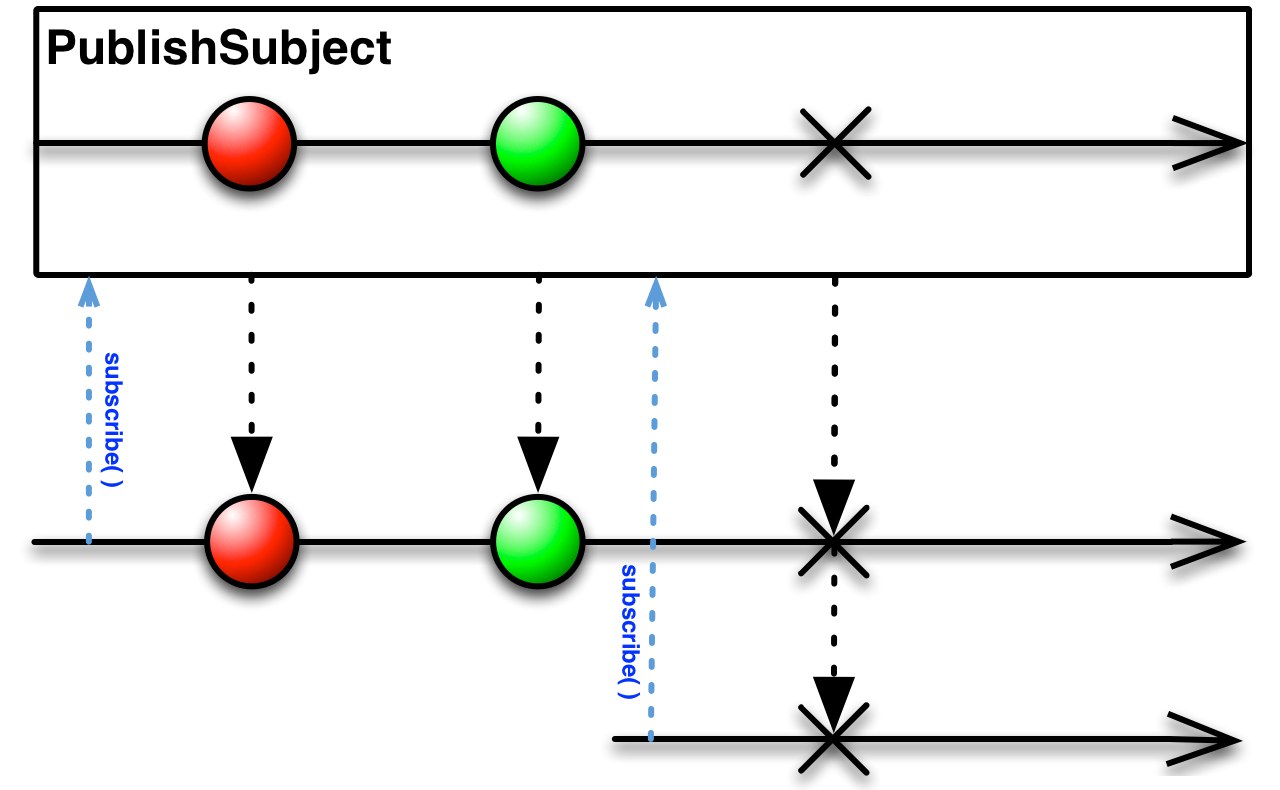
\includegraphics[scale=0.5]{imgs/pubsubj.png}
\caption{PublishSubject}
\end{figure}

\texttt{PublishSubject} emits to an observer only those items that are
emitted by the source Observable(s) \textbf{subsequent} to the time of
the subscription. This means that an observer will not receive the
previous emitted items.

\subsubsection{ReplaySubject}\label{replaysubject}

\begin{figure}[htbp]
\centering
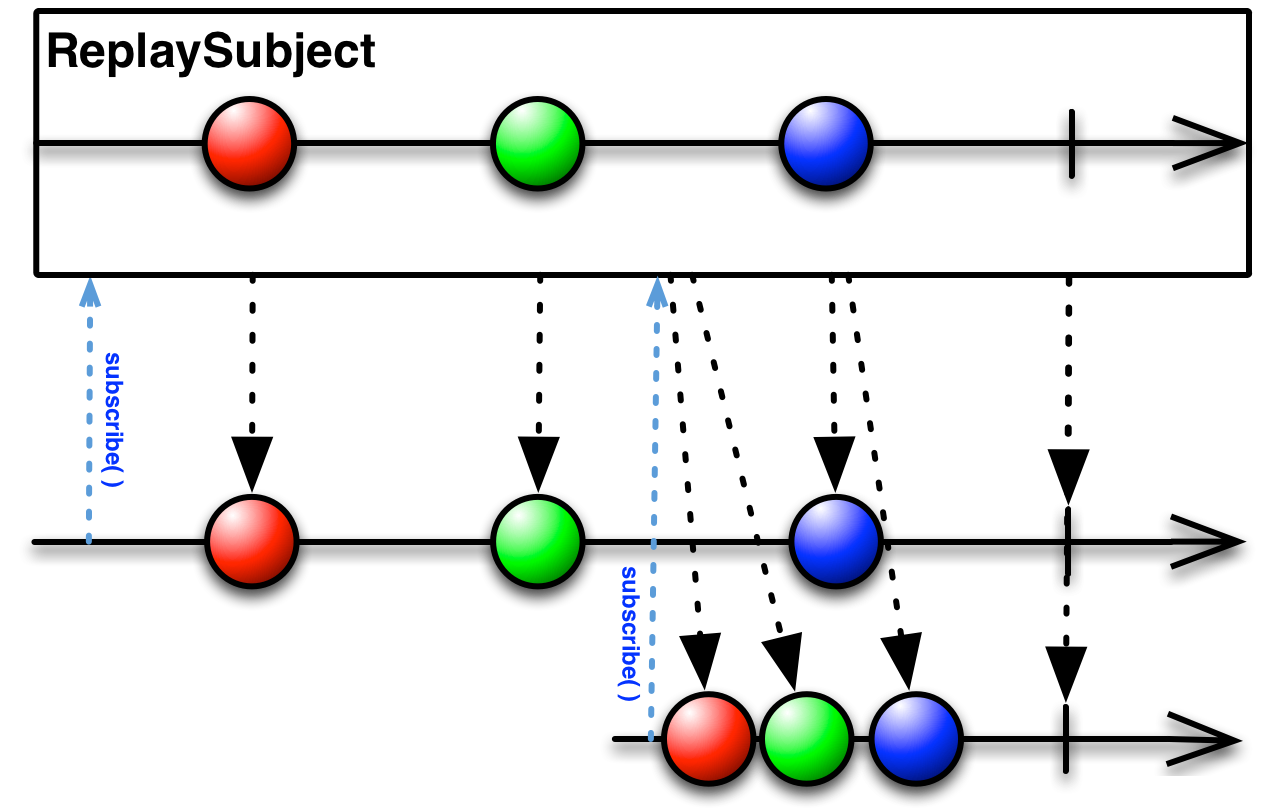
\includegraphics[scale=0.5]{imgs/replaysub.png}
\caption{ReplaySubject}
\end{figure}

\texttt{ReplaySubject} emits to any observer \textbf{all} of the items
that were emitted by the source Observable(s), regardless of when the
observer subscribes. To keep the memory consumption limited, this subject
also use a bounded buffer that enable to discard old items when the
limit size has been reached.

\subsubsection{AsyncSubject}\label{asyncsubject}

\begin{figure}[htbp]
\centering
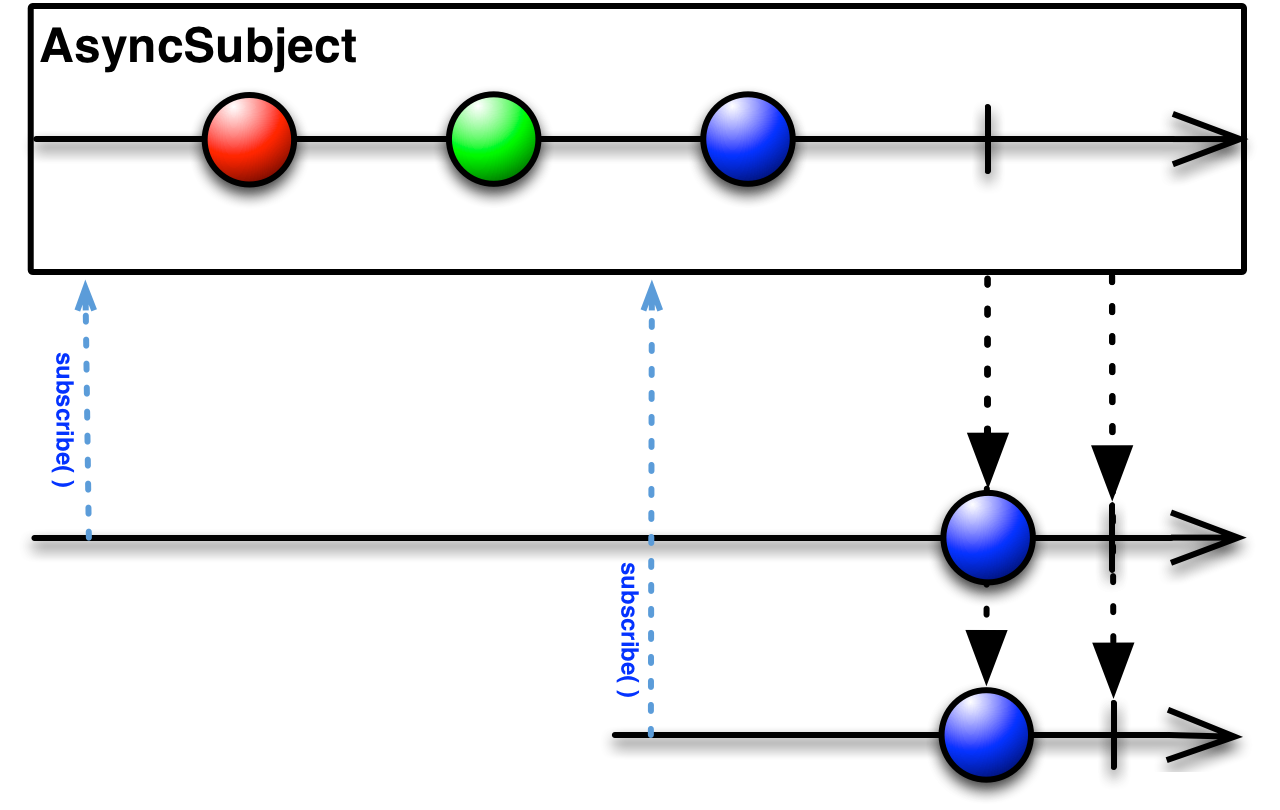
\includegraphics[scale=0.5]{imgs/asyncsubj.png}
\caption{AsyncSubject}
\end{figure}

An \texttt{AsyncSubject} caches and only remember the \textbf{last}
value of the Observable, and only after that source Observable completes
emits that value.

\subsubsection{BehaviorSubject}\label{behaviorsubject}

\begin{figure}[htbp]
\centering
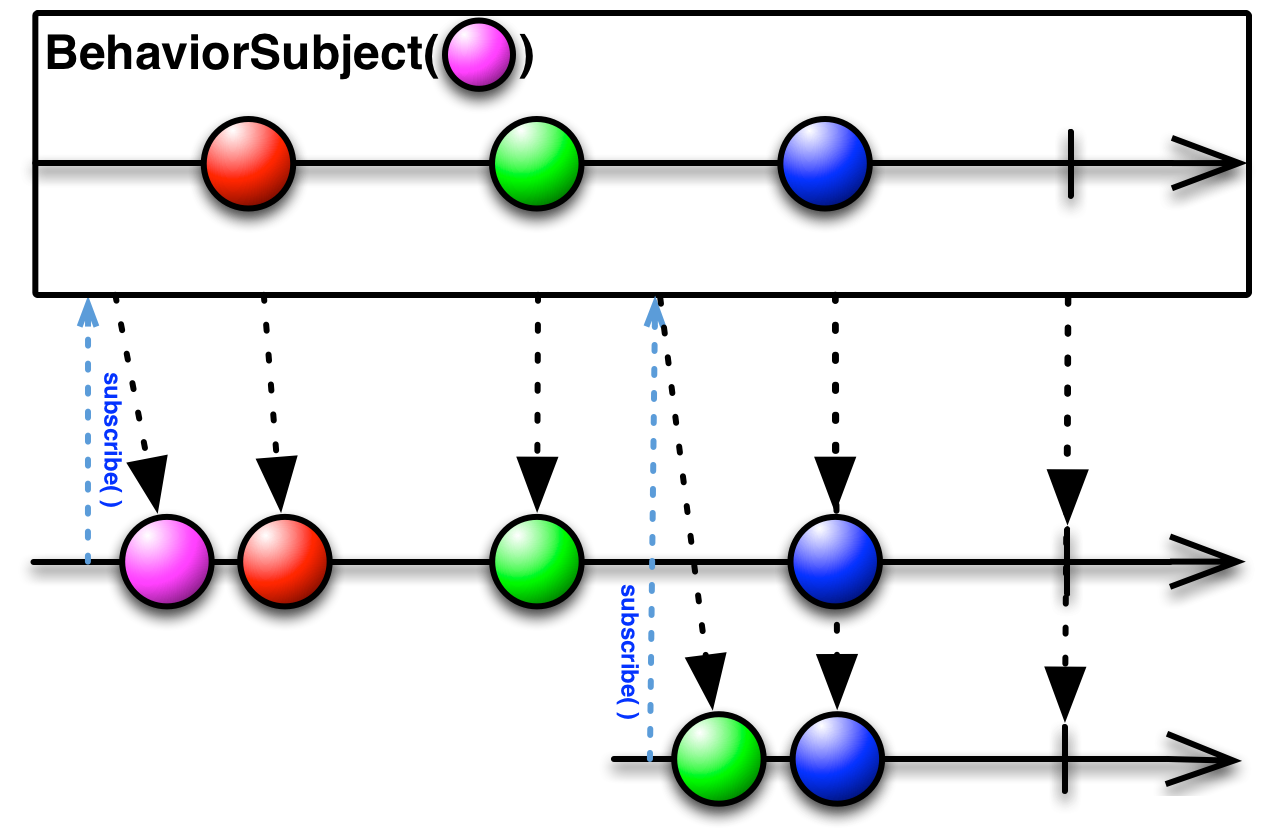
\includegraphics[scale=0.5]{imgs/behasubj.png}
\caption{BehaviorSubject}
\end{figure}

When an observer subscribes to a \texttt{BehaviorSubject}, it begins by
emitting the item most recently emitted by the source Observable (or a
seed/default value if none has yet been emitted) and then continues to
emit any other items emitted later by the source Observable(s).

In practice, it's really similar to the \textbf{Behavior} notion from
Elliot's FRP.

\subsection{RxAndroid}\label{rxandroid}

The previous sections cover all the main topic of RxJava. This section
will go a step further, introducing some additional features that bring
RxJava to the Android ecosystem.

\textbf{RxAndroid} is a separate module of RxJava that gives some
useful bindings to the developer.

The \texttt{AndroidSchedulers} package provides some specific scheduler
for the \emph{Android threading system}.

The additional schedulers provided are:

\begin{itemize}
\itemsep1pt\parskip0pt\parsep0pt
\item
  \texttt{AndroidSchedulers.mainThread(\ )}, that will execute an action
  on the main \textbf{Android UI thread}
\item
  \texttt{AndroidSchedulers.handlerThread(Handler\ handler)}, that
  \textbf{uses the provided Handler} to execute an action
\end{itemize}

A typical example of the usage of \texttt{mainThread(\ )} is the
following, that performs a download in the scheduler \texttt{io(\ )} and
the show the image to the user:

\begin{verbatim}
service.getImage(url)
.subscribeOn(Schedulers.io())
.observeOn(AndroidSchedulers.mainThread())
.subscribe(bitmap -> myImageView.setImageBitmap(bitmap));
\end{verbatim}

\textbf{ViewObservable} is another feature that adds some bindings for
android \texttt{View} that returns observables of events that come from
the UI, such as:

\begin{itemize}
\itemsep1pt\parskip0pt\parsep0pt
\item
  \texttt{clicks(\ )}, that emits a new item each time a \texttt{View}
  is \textbf{clicked}
\item
  \texttt{text(\ )}, that emits a new item each time a
  \texttt{TextView}'s \textbf{text content} is changed
\item
  \texttt{input(\ )}, same as above, for \texttt{CompoundButton}s
\item
  \texttt{itemClicks(\ )}, same as above, for \texttt{AdapterView}s
\end{itemize}

These methods are useful to bind the events from the user of an
application, reifying its action and reacting with some operation, in a
declarative way.

\section{ReactiveCocoa}\label{reactivecocoa}

\textbf{ReactiveCocoa} (RAC) is an opensource framework for FRP,
developed by Github for the \textbf{iOS} and \textbf{OS X} platforms.
RAC has been around for some years now. It started as an
\textbf{Objective-C} framework and now it's object of an almost-complete
rewrite using the brand new language introduced by Apple,
\textbf{Swift}.

At the time of writing (may/june/july 2015), RAC 3.0 is in beta. The 3.0
version offers new APIs in Swift, that are also mostly backward
compatible with version 2.0 (that is written in Objective-C).

Using Swift, the APIs now have a better and cleaner form. In fact, Swift
is a language that allows to build composable abstraction pretty easily,
supporting immutability (value types vs reference types), high-order
functions, optionals, custom operators, etc\ldots{}

In the community of iOS and OS X developers RAC is an emerging trend
that is clearly gaining the attention of an increasing number of users,
confirming the general trend of RP and FRP in our industry.


\subsection{Event and Signal}\label{event-and-signal}

The first abstraction that the framework introduces is the notion of
event. An \textbf{event} enables to account for \emph{discrete
phenomena}, and each of which has a stream (finite or infinite) of
occurrences. Each occurrence is a value paired with a time.
Events are considered to be improving list of occurrences. Or, in simpler
words, events are things that happen.

In RAC, events are first-class citizens, with the following type:

\begin{verbatim}
public enum Event<T, E: ErrorType> {
    case Next(Box<T>)
    case Error(Box<E>)
    case Completed
    case Interrupted
}
\end{verbatim}

The \texttt{Event} type, taken alone, doesn't say much. It's just an
enum with some possible related values.

\begin{quote}
In Swift, an enum is a value type that defines a common type for a group
of related values and enables you to work with those values in a
type-safe way within your code.
\end{quote}

The other fundamental type in RAC is the \texttt{Signal} type, defined
as:

\begin{verbatim}
public final class Signal<T, E: ErrorType>
\end{verbatim}

A signal is just a sequence of events in time that is conforms to the
grammar
\texttt{Next*\ (Error\ \textbar{}\ Completed\ \textbar{}\ Interrupted)?}.
The grammar introduces a precise semantics and clarify the meaning of
the concrete possible instances for the Event type:

\begin{itemize}
\itemsep1pt\parskip0pt\parsep0pt
\item
  \texttt{.Next} represents an event that carry information of a given
  type \texttt{T}
\item
  \texttt{.Error} represents an event that carry an error of a given
  type \texttt{E}
\item
  \texttt{.Completed} represents a successful terminal event
\item
  \texttt{.Interrupted} represents an event that indicates that the
  signal has been interrupted
\end{itemize}

Just like RxJava's Observable, also RAC's signal can be distincted in
two main categories: hot and cold signals. The main difference from
RxJava's implementation is that in RAC this fundamental distinction can
be found directly in the types. In fact, RAC defines \texttt{Signal}as
hot and \texttt{SignalProducer} as cold signals.

\emph{NB}: the previous introduction of Signal is general and applicable
on both Signal and SignalProducer.

The next sections will go deeper and explore more on Signals and
SignalProducers.

\subsubsection{Signal}\label{signal}

As introduced previously, Signal implements the abstraction of
\textbf{hot signal} as a signal that typically has \textbf{no start and
no end}.

A typical practical example for this type can be represented by the press
events of a button or the arrival of some notifications. They are just
events that happens with no relevance of the fact that someone is
observing them.

Using a popular philosophical metaphor:

\begin{quote}
If a tree falls in a forest and no one is around to hear it, \textbf{it
does make a sound}.
\end{quote}

Looking at the documentation, a Signal is defined as a \emph{push-driven
stream that sends Events over time}. Events will be sent to all
observers at the same time. So, if a Signal has different observers
subscribed to its events, every observer will always see the same
sequence of events.

The documentation says another crucial thing that clarifies the
modelling choice made by the developers:

\begin{quote}
Signals are generally used to represent event streams that are already
``in progress'', like notifications, user input, etc. To represent
streams that must first be \emph{started}, see the SignalProducer type.
\end{quote}

The RAC' maintainers decided to keep the distinction between hot and cold
Signal at the type level, so RAC offers both the \texttt{Signal} and
\texttt{SignalProducer} types.

The \texttt{Signal} type is defined as follows:

\begin{verbatim}
class Signal<T, E: ErrorType> {
  ...
}
\end{verbatim}

Signal is parameterized over \texttt{T}, the type of the events emitted
by the signal and \texttt{E}, the type that denotes the errors.

A Signal can be created by passing to the initializer a generator
closure, which is then invoked with a sink of type
\texttt{SinkOf\textless{}Event\textless{}String,\ NoError\textgreater{}\textgreater{}}.
The sink is then used by the closure to forward events to the Signal
through the \texttt{sendNext(\ )} method. A similar approach has been
implemented also by Akka Streams.

\textbf{In many cases, a stream of events that has no start and no end
can't terminate with an error.} A simple example of this case is a
stream of press events from a button. To overcome this possibility, RAC
introduces the type \texttt{NoError}, meaning that the signal can't
error out.

For the ``button example'', the type for the related signal might be
\texttt{Signal\textless{}Void,\ NoError\textgreater{}}, which means:

\begin{itemize}
\itemsep1pt\parskip0pt\parsep0pt
\item
  the user of the signal only cares about the occurrence of the event, no
  further information will be provided
\item
  the signal can't error out, since in this particular case it has no
  sense to model the fact that a button press can fail
\end{itemize}

The button example is just one of many others. If we consider the amount
of events that come from the UI, a lot of trivial examples come out
quickly:

\begin{itemize}
\itemsep1pt\parskip0pt\parsep0pt
\item
  a signal that models the changes of a text field
\item
  a signal that models the arrival of notifications (remote, local,
  etc\ldots{})
\item
  any other signal created combining other signals
\item
  \ldots{}
\end{itemize}

An example for the creation of a Signal is the following, taken from a
blog post of Colin Eberhardt, where a new String is produced every
second.

\begin{verbatim}
func createSignal() -> Signal<String, NoError> {
  var count = 0
  return Signal {
    sink in
    NSTimer.schedule(repeatInterval: 1.0) { timer in
      sendNext(sink, "tick #\(count++)")
    }
    return nil
  }
}
\end{verbatim}

To attach some side effect at each \texttt{Next}, \texttt{Error} or
\texttt{Completed} event that is produced by a \texttt{Signal}, an
observer has to register its interest using \textbf{observe}. The
\texttt{observe} operator accepts some closures or functions for any of
the event types the user of the API is interested in.

The real deal in using Signals is their power in term of declarativeness
when combining Signals with operators to create new Signals to work
with.

In RAC, all \textbf{operations} that can be applied to signals are
simply \textbf{free functions}, in contrast to the
``classical-method-definition-on-the-Signal-type approach''. As an
example, the \texttt{map} operator signature is defined as follows, with
the Signal on which the transformation will be applied passed as an
argument:

\begin{verbatim}
public func map<T, U, E>(transform: T -> U)
    (signal: Signal<T, E>) -> Signal<U, E> {
    ...
}
\end{verbatim}

To keep the APIs fluent RAC also introduces the pipe-forward operator
\texttt{\textbar{}\textgreater{}}, defined as follows:

\begin{verbatim}
public func |> <T, E, X>(signal: Signal<T, E>,
    transform: Signal<T, E> -> X) -> X {
    return transform(signal)
}
\end{verbatim}

The \texttt{\textbar{}\textgreater{}} operator doesn't do anything
special, since it only creates a specification.

RAC already offers a numbers of built in operators as free functions,
such as \texttt{combineLatest}, \texttt{zip}, \texttt{takeUntil},
\texttt{concat}, \ldots{}

A complete but simple example of usage of all of the aspects introduced
is the following:

\begin{verbatim}
createSignal()
  |> map { $0.uppercaseString }
  |> observe(next: { println($0) })
\end{verbatim}

The beauty of this approach is that the chain of operations fits the
types of each operation, so when the code compiles (and if the user of
the APIs has learned the semantics of each operators) the computation
acts as expected. All the relevant work for the newcomers of the
paradigm consist in taking the time needed to learn the basics and play
with the types and the operators.

\subsubsection{SignalProducer}\label{signalproducer}

The previous section introduced \texttt{Signal} as the type that
implements the ``hot signal'' abstraction. This section will cover the
other half of the story.

In RAC, \textbf{``cold signals''} are implemented with the
\texttt{SignalProducer} type, defined as follows:

\begin{verbatim}
public struct SignalProducer<T, E: ErrorType> {
    ...
}
\end{verbatim}

The generic types are the same as its ``hot'' counterpart, and also the
initializer is pretty similar, with a generator closure:

\begin{verbatim}
func createSignalProducer() -> SignalProducer<String, NoError> {
  var count = 0
  return SignalProducer {
    sink, disposable in
    NSTimer.schedule(repeatInterval: 0.1) { timer in
      sendNext(sink, "tick #\(count++)")
    }
  }
}
\end{verbatim}

Using a popular philosophical metaphor, again:

\begin{quote}
If a tree falls in a forest and no one is around to hear it, \textbf{it
doesn't make a sound}.
\end{quote}

Or, in other words, if no one subscribes to the SignalProducer, nothing
happens. For SignalProducer, the terminology for subscribing to its
events is \texttt{start(\ )}.

If more than one observer subscribe to the same SignalProducer, the
resources are allocated for each observer. In the example above, every
time an observer invoke the \texttt{start(\ )} method on the same
SignalProducer instance, a new instance of NSTimer is allocated.

Also on SignalProducers can be applied a wide range of operators. RAC
doesn't implement all the operators twice for Signal and SignalOperator,
but it offers a pipe-forward operator that lifts the operators and
transformation that can be applied to \texttt{Signal} to also operate on
\texttt{SignalProducer}.

The implementation of \texttt{\textbar{}\textgreater{}}, that applies on
the SignalProducer type using Signal's operator, is the following:

\begin{verbatim}
public func |> <T, E, U, F>(producer: SignalProducer<T, E>,
      transform: Signal<T, E> -> Signal<U, F>) -> SignalProducer<U, F> {
  return producer.lift(transform)
}
\end{verbatim}

\subsection{ProperyType}\label{properytype}

The previous sections introduced the abstractions that RAC offers to
describe signal. This section will introduce other collateral but
useful types.

\texttt{PropertyType} is a protocol that, when applied to a property,
\textbf{allows the observation of its changes}. Its definition is as
follows:

\begin{verbatim}
public protocol PropertyType {
    typealias Value

    var value: Value { get }
    var producer: SignalProducer<Value, NoError> { get }
}
\end{verbatim}

The semantics of this protocol is neat: - the \textbf{getter} return the
current value of the property - the \textbf{producer} return a producer
for Signals that will send the property's current value followed by all
changes over time

Starting from this protocol, RAC introduces: -
\texttt{ConstantProperty}, that represents a property that never change
- \texttt{MutableProperty}, that represents a mutable property -
\texttt{PropertyOf}, that represents a read-only view to a property

These types are really usefull when used in combination with the
\texttt{\textless{}\textasciitilde{}} operator, that binds properties
together. The bind operator comes in three flavors:

\begin{verbatim}
/// Binds a signal to a property, updating the property's
/// value to the latest value sent by the signal.
public func <~ <P: MutablePropertyType>(property: P, signal: 
	Signal<P.Value, NoError>) -> Disposable {}

/// Creates a signal from the given producer, which will 
/// be immediately bound to the given property, updating the 
/// property's value to the latest value sent by the signal.
public func <~ <P: MutablePropertyType>(property: P, 
	producer: SignalProducer<P.Value, NoError>) 
		-> Disposable { }

/// Binds `destinationProperty` to the latest values 
/// of `sourceProperty`.
public func <~ <Destination: MutablePropertyType, 
	Source: PropertyType where Source.Value == Destination.Value>
		(destinationProperty: Destination, 
			sourceProperty: Source) -> Disposable { }
\end{verbatim}

What these operators do is to create the wires that link each property
to each others, in a declarative manner. Each property is observable,
through its inner SignalProducer.


\subsection{Action}\label{action}

The last concept that RAC APIs introduce is the notion of
\texttt{Action}.

An action is something that will do some work in the future. An action
will be executed with an input and will return an output or an error.
Its type is generic, and it's exposed as:

\begin{verbatim}
public final class Action<Input, Output, Error: ErrorType>
\end{verbatim}

The constructor of an Action accepts a closure or a function that
creates a SignalProducer for each input, with the type
\texttt{Input\ -\textgreater{}\ SignalProducer\textless{}Output,\ Error\textgreater{})}.

A practical and useful use of Action is in conjunction with
\texttt{CocoaAction}, which is another type that wraps an Action for use
by a GUI control, with key-value observing, or with other Cocoa
bindings.


\section{Akka Streams}\label{akka-streams}

\textbf{Akka Streams} is a library that is developed on top akka actors,
and aims to provide a better tool for building \emph{ephemeral
transformation pipelines}.

Akka actors are used as a building block to build a higher abstraction.
Some of the biggest issues on building systems on untyped actor are the
following:

\begin{itemize}
\itemsep1pt\parskip0pt\parsep0pt
\item
  actors does \textbf{not compose} well
\item
  actors are \textbf{not} completely \textbf{type safe}
\item
  dealing with an high number of actors, with also a complex logic
  behind each behaviors, is really error prone and bring back an evil
  concept: global \textbf{state}.
\end{itemize}

An actor can be seen as a single \emph{unit of consistency}.

From the introduction of the documentation of akka streams:

\begin{quote}
Actors can be seen as dealing with streams as well: they send and
receive series of messages in order to transfer knowledge (or data) from
one place to another. We have found it tedious and error-prone to
implement all the proper measures in order to achieve stable streaming
between actors, since in addition to sending and receiving we also need
to take care to not overflow any buffers or mailboxes in the process.
Another pitfall is that Actor messages can be lost and must be
retransmitted in that case lest the stream have holes on the receiving
side. When dealing with streams of elements of a fixed given type,
Actors also do not currently offer good static guarantees that no wiring
errors are made: type-safety could be improved in this case.
\end{quote}

To overcome these issues, the developers behind Akka started developing
Akka Streams, a set of APIs that offers an intuitive and safe way to
build \textbf{stream processing pipelines}, with a particular attention
to efficiency and bounded resource usage.

Akka Streams is also conform to the Reactive Streams initiative (see the
appendix), and this means that the hard problem of propagating and
reacting to back-pressure has been incorporated in the design of Akka
Streams already, and also that Akka Streams interoperate seamlessly with
all other Reactive Streams implementations.

In Akka Streams, a linear processing pipeline can be expressed using the
following building blocks:

\begin{itemize}
\itemsep1pt\parskip0pt\parsep0pt
\item
  \textbf{Source}: A processing stage with exactly one output, emitting
  data elements whenever downstream processing stages are ready to
  receive them, respecting their demand.
\item
  \textbf{Sink}: A processing stage with exactly one input, signalling
  demand to the upstream and accepting data elements in response, as
  soon as they're produced.
\item
  \textbf{Flow}: A processing stage which has exactly one input and
  output, which connects its upstream and downstreams by transforming
  the data elements flowing through it.
\item
  \textbf{RunnableFlow}: A Flow that has both ends attached to a Source
  and Sink respectively, and is ready to be run().
\end{itemize}

The APIs also offer another core abstraction to build computation
graphs: 

\begin{itemize}
\itemsep1pt\parskip0pt\parsep0pt
\item
  \textbf{Graphs}: A processing stage with multiple flows
connected at a single point.
\end{itemize}

The next sections will depict all the core abstractions introduced here.


\subsection{Source}\label{source}

In Akka Streams, a \textbf{Source} is a set of stream processing steps
that has \textbf{one open output}. In Scala, the \texttt{Source} type is
defined as follows:

\begin{verbatim}
final class Source[Out]
\end{verbatim}

The \texttt{Out} type is the type of the elements the source produces.

It either can be an atomic source or it can comprise any number of
internal sources and transformation that are wired together. Some
examples of the former case is given from the following code, that shows
some of the utility constructor for the \texttt{Source} type.

\begin{verbatim}
// Create a source from an Iterable
Source(List(1, 2, 3))

// Create a source from a Future
Source(Future.successful("Hello Streams!"))

// Create a source from a single element
Source.single("only one element")

// an empty source
Source.empty
\end{verbatim}

An example of the latter case is when a \texttt{Flow} is attached to a
\texttt{Source}, resulting in a composite source, as in the following
example.

\begin{verbatim}
val tweets: Source[Tweet] = Source(...)
val filter: Flow[Tweet, Tweet] = Flow[Tweet].filter(
	t => t.hashtags.contains(hashtag))
val compositeSource: Source[Tweet] = tweets.via(filter)
\end{verbatim}

The \texttt{via(\ )} method transforms a source by appending the given
processing stages, and it's the glue that enables to build composite
sources.


\subsection{Sink}\label{sink}

The dual to the \texttt{Source} type is the \textbf{Sink} type, which
abstracts a set of stream processing steps that has one open input and
an attached output. In Scala the \texttt{Sink} type is defined as
follows:

\begin{verbatim}
final class Sink[In]
\end{verbatim}

The \texttt{In} type is the type of the elements the sink accepts.

It either can be an atomic sink or it can comprise any number of
internal sinks and transformation that are wired together. Some examples
of the former case is given from the following code, that shows some of
the utility constructor for the \texttt{Sink} type.

\begin{verbatim}
// Sink that folds over the stream and returns a Future
// of the final result as its materialized value
Sink.fold[Int, Int](0)(_ + _)

// Sink that returns a Future as its materialized value,
// containing the first element of the stream
Sink.head

// A Sink that consumes a stream without doing 
// anything with the elements
Sink.ignore

// A Sink that executes a side-effecting call for every 
// element of the stream
Sink.foreach[String](println(_))
\end{verbatim}

An example of the latter case is given by a Flow that is prepend to a
Sink to get a new composite sink, as in the following example:

\begin{verbatim}
val sum: Flow[(Long, Tweet), (Long, Tweet)] = 
	Flow[(Long, Tweet)].scan[(Long, Tweet)](0L, EmptyTweet)(
      (state, newValue) => (state._1 + 1L, newValue._2))
val out: Sink[(Long, Tweet)] = Sink.foreach[(Long, Tweet)]({
      case (count, tweet) => println(count + " Current tweet: " 
      	+ tweet.body + " -  " + tweet.author.handle)
    })

val compositeOut: Sink[(Long, Tweet)] = sum.to(out)
\end{verbatim}


\subsection{Flow and RunnableFlow}\label{flow-and-runnableflow}

The previous sections introduced the two ends of a computation. This
section will introduce the \textbf{Flow} abstraction: a processing stage
which has exactly one input and one output. In Scala, the \texttt{Flow}
type is defined as follows.

\begin{verbatim}
class Flow[In, Out]
\end{verbatim}

The \texttt{Out} type is the type of the elements the flow returns and
the \texttt{In} type is the type of the elements the flow accepts.

A \textbf{RunnableFlow} is a flow that has both ends attached to a
source and sink, and represents \emph{a flow that can run}. A trivial
example of \texttt{RunnableFlow} in action is the following:

\begin{verbatim}
val in: Source[Tweet] = Source(...)
val out: Sink[Tweet] = Sink.foreach(println)
val runnableFlow: RunnableFlow = in.to(out)

runnableFlow.run()
\end{verbatim}

As already introduced, Akka Streams implements an \emph{asynchronous
non-blocking back-pressure protocol} standardised by the Reactive
Streams specification, and the user doesn't have to manually manage
back-pressure handling code manually since this is already provided by
the library itself with a default implementation.

In this regards, there are two main scenarios: \textbf{slow publisher
with fast subscriber} and \textbf{fast publisher with slow subscriber}.

The best scenario is the former, where all the items produced by the
publisher are always delivered to the subscriber with no delay due to a
lack of demand. In fact, the protocol guarantees that the publisher will
never signal more items than the signalled demand, and since the
subscriber however is currently faster, it will be signalling demand at
a higher rate, so the publisher should not ever have to wait in
publishing its items. This scenario is also referred as \emph{push
mode}, since the publisher is never delayed in pushing items to the
subscriber.

The latter case if more problematic, since the subscriber is not able to
keep the pace of the publisher in accepting incoming items and needs to
signal its lack of demand to the publisher. Since the protocol
guarantees that the publisher will never signal more items than the
signalled demand, there the following strategies available:

\begin{itemize}
\itemsep1pt\parskip0pt\parsep0pt
\item
  not generate items, if it can control its production
\item
  buffering the items within a bounded queue, so the items can be
  provided when more demand is signalled
\item
  drop items until more demand is signalled
\item
  as an ultimate strategy, tear down the stream if none of the previous
  strategies are applicable
\end{itemize}

This latter scenario is also referred as \emph{pull mode}, since the
subriber drives the flow of items.

\subsection{Graph}\label{graph}

Since not every computation is or can be expressed as a linear
processing stage pipeline, Akka Streams also provide a graph-resembling
DSL for building stream processing graphs, in which each node can has
multiple inputs and outputs.

The documentation refers to graph operation as \textbf{junctions}, in
which multiple flows are connected at a single point, enabling to
perform any kind of \emph{fan-in} or \emph{fan-out}.

The Flow graph APIs provide a pretty straight forward abstraction:

\begin{itemize}
\itemsep1pt\parskip0pt\parsep0pt
\item
  \textbf{Flow}s represent the \textbf{connection} within the
  computation graph
\item
  \textbf{Junction}s represent the \textbf{fan-in and fan-out} point to
  which the flows are connected
\end{itemize}

The APIs already provide some of the most useful juctions, like the
following:

\begin{itemize}
\itemsep1pt\parskip0pt\parsep0pt
\item
  \texttt{Merge{[}In{]}} - \emph{(N inputs , 1 output)} picks randomly
  from inputs pushing them one by one to its output
\item
  \texttt{Zip{[}A,B{]}} -- \emph{(2 inputs, 1 output)} is a ZipWith
  specialised to zipping input streams of A and B into an (A,B) tuple
  stream
\item
  \texttt{Concat{[}A{]}} -- \emph{(2 inputs, 1 output)} concatenates two
  streams (first consume one, then the second one)
\item
  \texttt{Merge{[}In{]}} -- \emph{(N inputs , 1 output)} picks randomly
  from inputs pushing them one by one to its output
\item
  \texttt{Broadcast{[}T{]}} -- \emph{(1 input, N outputs)} given an
  input element emits to each output
\end{itemize}

The documentation also provide a simple but brilliant example that
illustrates how the DSL provided by the library can be used to express
graph computation keeping a great level of declarativeness and code
readability.

The following image shows a graph that expresses a computation in which:

\begin{itemize}
\itemsep1pt\parskip0pt\parsep0pt
\item
  \textbf{the edges are flows}
\item
  \textbf{the nodes are a sink, a source and two junctions}
\end{itemize}

\begin{figure}[htbp]
\centering
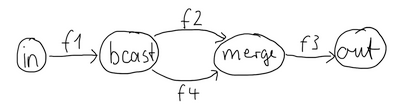
\includegraphics[scale=0.75]{imgs/graph.png}
\caption{A handwritten graph expressing a computation}
\end{figure}

The corresponding computation can be implemented as follows:

\begin{verbatim}
val g = FlowGraph.closed() { 
	implicit builder: FlowGraph.Builder[Unit] =>
  import FlowGraph.Implicits._
  val in = Source(1 to 10)
  val out = Sink.ignore
  val bcast = builder.add(Broadcast[Int](2))
  val merge = builder.add(Merge[Int](2))
  val f1, f2, f3, f4 = Flow[Int].map(_ + 10)
  in ~> f1 ~> bcast ~> f2 ~> merge ~> f3 ~> out
              bcast ~> f4 ~> merge
}
\end{verbatim}

When building and connecting each component, the compiler will check for
type correctness and this is a really useful things. The check to
control whether or not all elements have been properly connected is done
at run-time, though.

The framework also provides the notion of partial graph. A
\textbf{partial graph} is a graph with \emph{undefined sources, sinks or
both}, and it's useful to structure the code in different components,
that will be then connected with other components. In other words, the
usage of partial graphs favours code \textbf{composability}.

In many cases it's also possible to expose a complex graph as a simpler
structure, such as a Source, Sink or Flow, since these concepts can be
viewed as special cases of a partially connected graph:

\begin{itemize}
\itemsep1pt\parskip0pt\parsep0pt
\item
  a source is a partial flow graph with exactly one output
\item
  a sink is a partial flow graph with exactly one input
\item
  a Flow is a partial flow graph with exactly one input and exactly one
  output
\end{itemize}

One last feature that this section will depict and that Akka Stream
supports is the possibility to insert \textbf{cycles} in flow graphs.
This feature is potentially dangerous, since it may lead to deadlock or
liveness issues.

The problems quickly arise when there're unbalanced feedback loops in
the graph. Since Akka Stream is based on processing items in a bounded
manner, if a cycle has an unbounded number of items (for example, when
items always get reinjected in the cycle), the back-pressure will
deadlock the graph very quickly.

A possible strategy to avoid deadlocks in presence of \textbf{unbalanced
cycles} is introducing a \textbf{dropping element on the feedback arc},
that will drop items when back-pressure begins to act.

A brilliant example from the documentation is the following, where a
\texttt{buffer(\ )} is used with a 10 items capacity and a
\texttt{dropHead} strategy.

\begin{verbatim}
FlowGraph.closed() { implicit b =>
  import FlowGraph.Implicits._
  val merge = b.add(Merge[Int](2))
  val bcast = b.add(Broadcast[Int](2))

  source ~> merge ~> Flow[Int].map { 
			s => println(s); s } ~> bcast ~> Sink.ignore
      merge <~ Flow[Int].buffer(10, OverflowStrategy.dropHead) <~ bcast
}
\end{verbatim}

An alternative approach in solving the problem is by \textbf{building a
cycle that is balanced from the beginning}, by using \textbf{junctions
that balance the inputs}. Thus, the previous example can also be solved
in the following manner, with:

\begin{itemize}
\itemsep1pt\parskip0pt\parsep0pt
\item
  a \texttt{ZipWith(\ )} junction, that will balance the feedback loop
  with the source
\item
  a \texttt{Concat(\ )} combined with another \texttt{Source(\ )} with
  an initial element that performs an initial ``kick-off''. In fact,
  using a balancing operator to balance a feedback loops require an
  initial element in the feedback loop, otherwise we fall in the
  ``chicken-and-egg'' problem.
\end{itemize}

\begin{verbatim}
FlowGraph.closed() { implicit b =>
  import FlowGraph.Implicits._
  val zip = b.add(ZipWith((left: Int, right: Int) => left))
  val bcast = b.add(Broadcast[Int](2))
  val concat = b.add(Concat[Int]())
  val start = Source.single(0)

  source ~> zip.in0
  zip.out.map { s => println(s); s } ~> bcast ~> Sink.ignore
  zip.in1 <~ concat <~ start
             concat         <~          bcast
}
\end{verbatim}
